 \documentclass[9pt]{beamer}
%\documentclass[compress,9pt,usenames,dvipsnames]{beamer}
% \usepackage[utf8]{inputenc}
% \includeonlyframes{current}
\setbeamercovered{dynamic}
\usepackage{etex}
\usepackage{graphicx,url,psfrag}
\usepackage{tikz}
\usetikzlibrary{decorations.pathreplacing,calc,decorations.fractals,through,shapes,patterns,arrows.meta,decorations.pathreplacing,arrows,shapes,}
\usepackage{tikzpeople}
% \usepackage[center]{subfigure}
\usepackage{enumerate}
\usepackage[makeroom]{cancel}
\usepackage{mathtools}
\usepackage{graphbox}
\usepackage{amssymb}
\usepackage{comment}
\excludecomment{codes}
% \usepackage{movie15}
% \usepackage[showframe]{geometry}
% \usepackage{enumitem}

%
% for warning sign
%
\usepackage{pgfplots}
\usepackage{stackengine}
\usepackage{scalerel}
\usepackage{xcolor}
\usepackage{dbt}
\newcommand\dangersign[1][2ex]{%
  \renewcommand\stacktype{L}%
  \scaleto{\stackon[1.3pt]{\color{red}$\triangle$}{\tiny !}}{#1}%
}
% %  The following is to show codes:
\usepackage{listings}
% \usepackage{color}

\usepackage{pifont}% http://ctan.org/pkg/pifont
\newcommand{\cmark}{\ding{51}}%
\newcommand{\xmark}{\ding{55}}%

\definecolor{dkgreen}{rgb}{0,0.6,0}
\definecolor{gray}{rgb}{0.5,0.5,0.5}
\definecolor{mauve}{rgb}{0.58,0,0.82}

\lstset{frame=tb,
  language=Java,
  aboveskip=3mm,
  belowskip=3mm,
  showstringspaces=false,
  columns=flexible,
  basicstyle={\small\ttfamily},
  numbers=none,
  numberstyle=\tiny\color{gray},
  keywordstyle=\color{blue},
  commentstyle=\color{dkgreen},
  stringstyle=\color{mauve},
  breaklines=true,
  breakatwhitespace=true,
  tabsize=3
}
\lstset{language=Python}

\lstset{ %
  language=Python,                     % the language of the code
  basicstyle=\footnotesize,       % the size of the fonts that are used for the code
  numbers=left,                   % where to put the line-numbers
  numberstyle=\tiny\color{gray},  % the style that is used for the line-numbers
  stepnumber=1,                   % the step between two line-numbers. If it's 1, each line
                                  % will be numbered
  numbersep=5pt,                  % how far the line-numbers are from the code
  backgroundcolor=\color{black},  % choose the background color. You must add \usepackage{color}
  showspaces=false,               % show spaces adding particular underscores
  showstringspaces=false,         % underline spaces within strings
  showtabs=false,                 % show tabs within strings adding particular underscores
  frame=single,                   % adds a frame around the code
  rulecolor=\color{black},        % if not set, the frame-color may be changed on line-breaks within not-black text (e.g. commens (green here))
  tabsize=2,                      % sets default tabsize to 2 spaces
  captionpos=b,                   % sets the caption-position to bottom
  breaklines=true,                % sets automatic line breaking
  breakatwhitespace=false,        % sets if automatic breaks should only happen at whitespace
  title=\lstname,                 % show the filename of files included with \lstinputlisting;
                                  % also try caption instead of title
  keywordstyle=\color{blue},      % keyword style
  commentstyle=\color{dkgreen},   % comment style
  stringstyle=\color{mauve},      % string literal style
  escapeinside={\%*}{*)},         % if you want to add a comment within your code
  morekeywords={*,...}            % if you want to add more keywords to the set
}
% \usepackage[usenames,dvipsnames]{color}
% \lstset{
%   language=R,                     % the language of the code
%   basicstyle=\tiny\ttfamily, % the size of the fonts that are used for the code
%   numbers=left,                   % where to put the line-numbers
%   numberstyle=\tiny\color{Blue},  % the style that is used for the line-numbers
%   stepnumber=1,                   % the step between two line-numbers. If it is 1, each line
%                                   % will be numbered
%   numbersep=5pt,                  % how far the line-numbers are from the code
%   backgroundcolor=\color{white},  % choose the background color. You must add \usepackage{color}
%   showspaces=false,               % show spaces adding particular underscores
%   showstringspaces=false,         % underline spaces within strings
%   showtabs=false,                 % show tabs within strings adding particular underscores
%   frame=single,                   % adds a frame around the code
%   rulecolor=\color{black},        % if not set, the frame-color may be changed on line-breaks within not-black text (e.g. commens (green here))
%   tabsize=2,                      % sets default tabsize to 2 spaces
%   captionpos=b,                   % sets the caption-position to bottom
%   breaklines=true,                % sets automatic line breaking
%   breakatwhitespace=false,        % sets if automatic breaks should only happen at whitespace
%   keywordstyle=\color{RoyalBlue},      % keyword style
%   commentstyle=\color{YellowGreen},   % comment style
%   stringstyle=\color{ForestGreen}      % string literal style
% }

% \usepackage[dvipsnames]{xcolor}
% \newcommand{\Cross}{\mathbin{\tikz [x=1.4ex,y=1.4ex,line width=.2ex] \draw (0,0) -- (1,1) (0,1) -- (1,0);}}%
\newcommand{\Crossme}[1]{\!\!
\tikz [black,x=1.1em,y=1.1em,line width=.4ex]
\draw (-0.5,-0.5) -- (0,0) node {\footnotesize #1} -- (0.5,0.5) (0.5,-0.5) -- (-0.5,0.5);}%
\newcommand{\Checkme}[1]{\!\!
\tikz [x=1.1em,y=1.1em,line width=.4ex]
\draw [black] (0,0.7) -- (0.3,0) --(0.9,1.0) (0.5,0.5) node {\footnotesize #1};}
% \beamerdefaultoverlayspecification{<+-| alert@+>} %(this will show line by line)
\beamerdefaultoverlayspecification{<+->} %(this will show line by

% \usepackage{natbib}
% \input{../myMathSymbols.tex}
% \newcommand{\tlMr}[4]{\:{}^{\hspace{0.2em}#1}_{#2} \hspace{-0.1em}#3_{#4}}

% Smiley face\Smiley{} \Frowny{}
\usepackage{marvosym}
% -------------------------------------------------
%  Set directory for figs
% -------------------------------------------------
\usepackage{grffile}
\graphicspath{{Codes/}}
% -------------------------------------------------
%  Define colors
% -------------------------------------------------
\def\refcolor{cyan}
\def\excolor{brown}
% \usepackage{color}
% \usepackage[dvipsnames]{xcolor}


% % % Define danger sign
\newcommand*{\TakeFourierOrnament}[1]{{%
\fontencoding{U}\fontfamily{futs}\selectfont\char#1}}
\newcommand*{\danger}{\TakeFourierOrnament{66}}


% -------------------------------------------------
%  Define short-hand symbols.
% -------------------------------------------------
\newcommand{\B}{\textbf{B}}
\newcommand{\PP}{\mathbb{P}}
\newcommand{\E}{\mathbb{E}}
\newcommand{\D}{\mathbb{D}}
\newcommand{\W}{\dot{W}}
\newcommand{\ud}{\ensuremath{\mathrm{d}}}
\newcommand{\Ceil}[1]{\left\lceil #1 \right\rceil}
\newcommand{\Floor}[1]{\left\lfloor #1 \right\rfloor}
\newcommand{\sgn}{\text{sgn}}
\newcommand{\Lad}{\text{L}_{\text{ad}}^2}
\newcommand{\SI}[1]{\mathcal{I}\left[#1 \right]}
\newcommand{\SIB}[2]{\mathcal{I}_{#2}\left[#1 \right]}
\newcommand{\Indt}[1]{1_{\left\{#1 \right\}}}
\newcommand{\LadInPrd}[1]{\left\langle #1 \right\rangle_{\text{L}_\text{ad}^2}}
\newcommand{\LadNorm}[1]{\left|\left|  #1 \right|\right|_{\text{L}_\text{ad}^2}}
\newcommand{\Norm}[1]{\left|\left|  #1   \right|\right|}
\newcommand{\Ito}{It\^{o} }
\newcommand{\Itos}{It\^{o}'s }
\newcommand{\spt}[1]{\text{supp}\left(#1\right)}
\newcommand{\InPrd}[1]{\left\langle #1 \right\rangle}
\newcommand{\mr}{\textbf{r}}
\newcommand{\Ei}{\text{Ei}}
\newcommand{\arctanh}{\operatorname{arctanh}}
\newcommand{\ind}[1]{\mathbb{I}_{\left\{ {#1} \right\} }}
\newcommand{\Var}{\text{Var}}
\newcommand{\Cov}{\text{Cov}}
\newcommand{\Corr}{\text{Corr}}

\newcommand{\baseurl}[1]{\footnotesize\url{http://math.emory.edu/~lchen41/teaching/2020_Spring/#1}}


\newcommand*\mystrut[1]{\vrule width0pt height0pt depth#1\relax} % adding vertical space

\DeclareMathOperator{\esssup}{\ensuremath{ess\,sup}}

\newcommand{\steps}[1]{\vskip 0.3cm \textbf{#1}}
\newcommand{\calB}{\mathcal{B}}
\newcommand{\calC}{\mathcal{C}}
\newcommand{\calD}{\mathcal{D}}
\newcommand{\calE}{\mathcal{E}}
\newcommand{\calF}{\mathcal{F}}
\newcommand{\calG}{\mathcal{G}}
\newcommand{\calK}{\mathcal{K}}
\newcommand{\calH}{\mathcal{H}}
\newcommand{\calI}{\mathcal{I}}
\newcommand{\calL}{\mathcal{L}}
\newcommand{\calM}{\mathcal{M}}
\newcommand{\calN}{\mathcal{N}}
\newcommand{\calO}{\mathcal{O}}
\newcommand{\calT}{\mathcal{T}}
\newcommand{\calP}{\mathcal{P}}
\newcommand{\calR}{\mathcal{R}}
\newcommand{\calS}{\mathcal{S}}
\newcommand{\calV}{\mathcal{V}}
\newcommand{\bbC}{\mathbb{C}}
\newcommand{\bbN}{\mathbb{N}}
\newcommand{\bbP}{\mathbb{P}}
\newcommand{\bbZ}{\mathbb{Z}}
\newcommand{\myVec}[1]{\overrightarrow{#1}}
\newcommand{\sincos}{\begin{array}{c} \cos \\ \sin \end{array}\!\!}
\newcommand{\CvBc}[1]{\left\{\:#1\:\right\}}
\newcommand*{\one}{{{\rm 1\mkern-1.5mu}\!{\rm I}}}

\newcommand{\OneFrame}[1]{
\begin{enumerate}\item[#1] \phantom{av} \\[20em]\vfill\phantom{av}\myEnd\end{enumerate}}

\newcommand{\bH}{\ensuremath{\mathrm{H}}}
\newcommand{\Ai}{\ensuremath{\mathrm{Ai}}}

\newcommand{\R}{\mathbb{R}}
\newcommand{\myEnd}{\hfill$\square$}
\newcommand{\ds}{\displaystyle}
\newcommand{\Shi}{\text{Shi}}
\newcommand{\Chi}{\text{Chi}}
\newcommand{\Erf}{\ensuremath{\mathrm{erf}}}
\newcommand{\Erfc}{\ensuremath{\mathrm{erfc}}}
\newcommand{\He}{\ensuremath{\mathrm{He}}}
\newcommand{\Res}{\ensuremath{\mathrm{Res}}}

\newcommand{\mySeparateLine}{\begin{center}
 \makebox[\linewidth]{\rule{0.6\paperwidth}{0.4pt}}
\end{center}}

\theoremstyle{definition}
% \newtheorem{definition}[theorem]{Definition}
% \newtheorem{hypothesis}[theorem]{Hypothesis}
\newtheorem{assumption}[theorem]{Assumption}

\theoremstyle{plain}
% \newtheorem{theorem}{Theorem}
% \newtheorem{corollary}[theorem]{Corollary}
% \newtheorem{lemma}[theorem]{Lemma}
\newtheorem{proposition}[theorem]{Proposition}

\mode<presentation>
{
%      \usetheme{Warsaw}
%     \usetheme{JuanLesPins}
%  \usetheme{Hannover}
%  \usetheme{Montpellier}
   \useoutertheme{default}
  % or ...

  \setbeamercovered{transparent}
  % or whatever (possibly just delete it)
 \setbeamertemplate{frametitle}{
  \begin{centering}
    \color{blue}
    {\insertframetitle}
    \par
  \end{centering}
  }
}
\usefoottemplate{\hfill \insertframenumber{}}
% \inserttotalframenumber

\usepackage[english]{babel}
% or whatever

% \usepackage[latin1]{inputenc}
% or whatever

\usepackage{times}
\usepackage[T1]{fontenc}
% Or whatever. Note that the encoding and the font should match. If T1
% does not look nice, try deleting the line with the fontenc.

% \DeclareMathOperator{\Lip}{Lip}
\DeclareMathOperator{\lip}{l}
% \DeclareMathOperator{\Vip}{\overline{v}}
% \DeclareMathOperator{\vip}{\underline{v}}
% \DeclareMathOperator{\vv}{v}
% \DeclareMathOperator{\BC}{BC}
% \DeclareMathOperator{\CH}{CD}

\usepackage{pgfpages}
% \setbeameroption{show notes}
% \setbeamertemplate{note page}[plain]
% \setbeameroption{second mode text on second screen=right}
% \setbeameroption{show notes on second screen=right}
%

% Delete this, if you do not want the table of contents to pop up at
% the beginning of each subsection:
% \AtBeginSubsection[]
% {
%   \begin{frame}<beamer>{Outline}
%     \tableofcontents[currentsection,currentsubsection]
%   \end{frame}
% }

% If you wish to uncover everything in a step-wise fashion, uncomment
% the following command:
% \beamerdefaultoverlayspecification{<+->}

% % % % % % % % % % % % % % % % % % %
%  Define a block
% % % % % % % % % % % % % % % % % % %
\newenvironment<>{problock}[1]{%
  \begin{actionenv}#2%
      \def\insertblocktitle{#1}%
      \par%
      \mode<presentation>{%
        \setbeamercolor{block title}{fg=white,bg=olive!95!black}
       \setbeamercolor{block body}{fg=black,bg=olive!25!white}
       \setbeamercolor{itemize item}{fg=white!20!white}
       \setbeamertemplate{itemize item}[triangle]
     }%
      \usebeamertemplate{block begin}}
    {\par\usebeamertemplate{block end}\end{actionenv}}

\newenvironment<>{assblock}[1]{%
  \begin{actionenv}#2%
      \def\insertblocktitle{#1}%
      \par%
      \mode<presentation>{%
        \setbeamercolor{block title}{fg=white,bg=green!50!black}
       \setbeamercolor{block body}{fg=black,bg=green!10}
       \setbeamercolor{itemize item}{fg=green!80!black}
       \setbeamertemplate{itemize item}[triangle]
     }%
      \usebeamertemplate{block begin}}
    {\par\usebeamertemplate{block end}\end{actionenv}}


% \newtheorem{proofnoend}{Proof.}
% \AtBeginEnvironment{proofnoend}{%
%   \setbeamercolor{block title}{use=example text,fg=lgtblue,bg=background}
%   % \setbeamercolor{block body}{parent=normal text,use=block title example,fg=yellow}
% }

% Define some colors
\definecolor{white}{HTML}{FFFFFF}              % #FFFFFF
\definecolor{pink}{HTML}{FB73BE}               % #FB73BE
\definecolor{coral}{HTML}{FF8D71}              % #FF8D71
\definecolor{yellow}{HTML}{FFE066}             % #FFE066
\definecolor{teal}{HTML}{59F3CE}               % #59F3CE
\definecolor{lgtblue}{HTML}{65D0FA} 	       % #65D0FA
\definecolor{blue}{HTML}{4984F2}               % #4984F2
\definecolor{purple}{HTML}{A87DFF}             % #A87DFF
\definecolor{red}{HTML}{FF3d30}                % #FF3d30
% \definecolor{magenta}{HTML}{FF80FF}                % #FF3d30
\definecolor{green}{HTML}{BBFFB9}              % #BBFFB9
% \definecolor{green}{HTML}{59F3CE}              % #BBFFB9
\setbeamercolor{alerted text}{fg=red}
% \setbeamercolor{block title}{bg=background,fg=lgtblue}

\setbeamercolor{section in toc}{fg=yellow}
\setbeamercolor{subsection in toc}{fg=red}

% \newtheorem{myexample}{\it Example}[section]
\newcounter{myexample}[section]
\resetcounteronoverlays{myexample}
\newenvironment{myexample}[1][]{\refstepcounter{myexample}\par\medskip
\noindent \textbf{\textcolor{green}{Example~\mySecNum-\themyexample~#1}} \rmfamily}{\medskip}

\newcounter{mydefinition}[section]
\resetcounteronoverlays{mydefinition}
\newenvironment{mydefinition}[1][]{\refstepcounter{mydefinition}\par\medskip
\noindent \textbf{\textcolor{yellow}{Definition~\mySecNum-\themydefinition~#1}} \rmfamily}{\medskip}

% \NewCommandCopy{\oldref}{\ref}
% \let\oldref\ref
\newcommand{\myref}[1]{\mySecNum-\ref{#1}}

\newcounter{remark}[section]
\resetcounteronoverlays{remark}
\newenvironment{remark}[1][]{\refstepcounter{remark}\par\medskip
\noindent \textbf{\textcolor{blue}{Remark~\mySecNum-\theremark~#1}} \rmfamily}{\medskip}

\newcounter{mythm}[section]
\resetcounteronoverlays{mythm}
\newenvironment{mythm}[1][]{\refstepcounter{mythm}\par\medskip
\noindent \textbf{\textcolor{lgtblue}{Theorem~\mySecNum-\themythm~#1}} \rmfamily}{\medskip}

\newenvironment{mycor}[1][]{\refstepcounter{mythm}\par\medskip
\noindent \textbf{\textcolor{lgtblue}{Corollary~\mySecNum-\themythm~#1}} \rmfamily}{\medskip}

% \newtheorem{solution}{\textcolor{purple}{Solution}}
\newenvironment{mysol}[1][]{\par\medskip
\noindent \textbf{\textcolor{purple}{Solution#1.~}} \rmfamily}{\medskip}

\newenvironment{myproof}[1][]{\par\medskip
\noindent \textbf{\textcolor{purple}{Proof#1.~}} \rmfamily}{\medskip}

\long\def\script#1{}

% \numberwithin{equation}{section}

% If you have a file called "university-logo-filename.xxx", where xxx
% is a graphic format that can be processed by latex or pdflatex,
% resp., then you can add a logo as follows:

% \pgfdeclareimage[height=1cm]{Emory}{figs/Emory.png}


\title % (optional, use only with long paper titles)
{
  Financial Mathematics \\
  \bigskip
  \small MATH 5870/6870\footnote{\textcolor{gray}{Based on Robert L. McDonald's {\it Derivatives Markets}, 3rd Ed, Pearson, 2013.}}\\
  Fall 2021
}

% \subtitle
% {Research Plan} % (optional)

\author{Le Chen\\[1em]
  {\small\textcolor{gray}{\url{lzc0090@auburn.edu}}}
}


\institute[Auburn University]
{
% \pgfuseimage{Emory}\\[3em]
% {\small Auburn University}\\[1em]
% {\small Auburn AL}\\[3em]
\textcolor{gray}{Last updated on } \\[1em]
\textcolor{gray}{\today}
 \vspace{8em}
}
% - Use the \inst command only if there are several affiliations.
% - Keep it simple, no one is interested in your street address.

\date[Auburn]{Auburn University\\ \textcolor{gray}{Auburn AL}}
% \date{}

% \subject{}



\begin{document}
\begin{frame}[noframenumbering]
  \titlepage
\end{frame}
\newcommand{\myChapter}{Chapter 9. Parity and other option relationships}
\newcommand{\mySection}[1]{
  \section{\S\: #1}
  \begin{frame}{\myChapter}\tableofcontents\end{frame}
  \begin{frame}{\myChapter}\tableofcontents[currentsection]\end{frame}
  }
\begin{frame}
\begin{center}
\huge
\myChapter
\end{center}
\end{frame}
\def\mySecNum{9.1}
\mySection{\mySecNum~Put-call parity}
%-------------- start slide -------------------------------%{{{ 1
\begin{frame}[fragile]
\begin{center}
	How does one value the right to back away from a commitment?
	\bigskip

	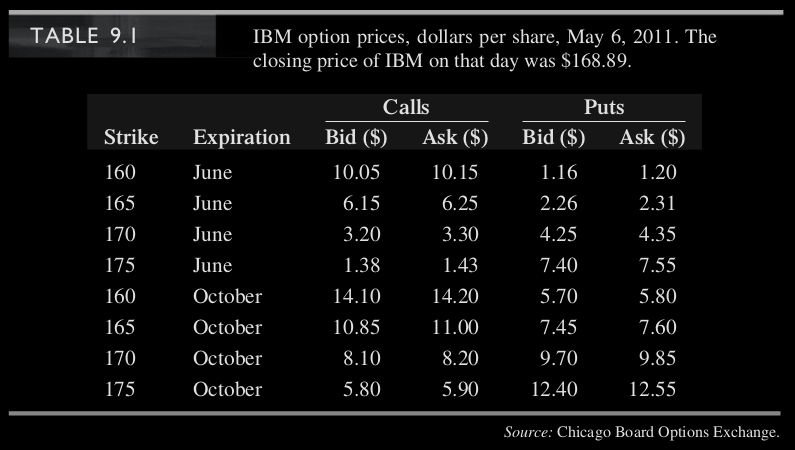
\includegraphics[scale=0.25]{figs/Table-9-1.png}
\end{center}
\end{frame}
%-------------- end slide -------------------------------%}}}
%-------------- start slide -------------------------------%{{{ 1
\begin{frame}[fragile,t]
	\begin{itemize}
		\item What determines the difference between put and call prices at a given strike?
		\item How would the premiums change if these options were European rather than American?
		\item It appears that, for a given strike, the October options are more expensive than the June options. Is this necessarily true?
		\item Do call premiums always decrease as the strike price increases? Do put premiums always increase as the strike price increases?
		\item Both call and put premiums change by less than the change in the strike price. Does this always happen?
	\end{itemize}
\end{frame}
%-------------- end slide -------------------------------%}}}
%-------------- start slide -------------------------------%{{{ 1
\begin{frame}[fragile,t]
	\frametitle{European options}

	\begin{align*}
		C(K,T) - P(K,T) & = \text{PV}_{0,T} \left(F_{0,T}-K\right) \\
                    & = e^{-rT}\left(F_{0,T}-K\right)
	\end{align*}

	\pause
	\bigskip
	\begin{center}
		Buying a call and selling a put \\
		with the strike both equal to the forward price (i.e., $K=F_{0,T}$)\\
		creates a synthetic forward contract \\
		and hence must have a zero price.

		\pause
		\bigskip
		\mySeparateLine
		\bigskip

		Parity generally fails for American options!
	\end{center}
\end{frame}
%-------------- end slide -------------------------------%}}}
%-------------- start slide -------------------------------%{{{ 1
\begin{frame}[fragile,t]
	\frametitle{Parity for stocks}
	\begin{align*}
		C(K,T) = P(K,T) + \left(S_0-\text{PV}_{0,T}(\text{Div})\right) - e^{-rT} K
	\end{align*}
\end{frame}
%-------------- end slide -------------------------------%}}}
%-------------- start slide -------------------------------%{{{ 1
\begin{frame}[fragile,t]
	\begin{myexample}
		\label{Eg:9-1}
		Suppose that the price of a non-dividend-paying stock is \$40, the continuously compounded
		interest rate is 8\%, and options have 3 months to expiration. If a 40-strike European call
		sells for \$2.78, find the price for a 40-strike European put sells.
	\end{myexample}
	\bigskip
	\pause
	\begin{mysol}
		Let the price for put be $y$. Then
		\begin{align*}
			\$2.78 = y + \$40 - \$40e^{−0.08\times0.25}
		\end{align*}
		Hence,
		\begin{align*}
			y = \$1.99.
		\end{align*}
		\myEnd
	\end{mysol}
\end{frame}
%-------------- end slide -------------------------------%}}}
%-------------- start slide -------------------------------%{{{ 1
\begin{frame}[fragile,t]
	\begin{center}
		Why is a call more expensive than a put?

		\pause
		\bigskip
		\mySeparateLine
		\bigskip

		When $S_0=K$ and $\text{Div}=0$, then
		\begin{align*}
			C(K,T)-P(K,T) = K \left(1-e^{-rT}\right)
		\end{align*}
		\bigskip

		\pause
		The difference of a call and put is\\
		the \textcolor{cyan}{time value of money}.
	\end{center}
\end{frame}
%-------------- end slide -------------------------------%}}}
%-------------- start slide -------------------------------%{{{ 1
\begin{frame}[fragile,t]
	\begin{myexample}
Make the same assumptions as in Example \myref{Eg:9-1}, except suppose that the
stock pays a \$5 dividend just before expiration. If the price of the European call is \$0.74, what
would be the price of the European put?
	\end{myexample}
	\bigskip
	\pause
	\begin{mysol}
		Let the price for put be $y$. Then
		\begin{align*}
			\$0.74 = y + \left(\$40 - \$5 e^{-0.08 \times 0.25}\right) - \$40e^{−0.08\times0.25}
		\end{align*}
		Hence,
		\begin{align*}
			y = \$4.85.
		\end{align*}
		\myEnd
	\end{mysol}
\end{frame}
%-------------- end slide -------------------------------%}}}
%-------------- start slide -------------------------------%{{{ 1
\begin{frame}[fragile,t]
	\frametitle{Synthetic securities}
	\begin{align*}
		C(K,T) = P(K,T) + \left(S_0-\text{PV}_{0,T}(\text{Div})\right) - e^{-rT} K
	\end{align*}
	\mySeparateLine

	\begin{itemize}
		\item \textcolor{magenta}{Synthetic stock}
			\begin{align*}
				\textcolor{magenta}{S_0} = C(K,T) - P(K,T) + \text{PV}_{0,T}\left(\text{Div}\right) + e^{-rT} K
			\end{align*}
	\end{itemize}
\end{frame}
%-------------- end slide -------------------------------%}}}
%-------------- start slide -------------------------------%{{{ 1
\begin{frame}[fragile,t]
	\begin{align*}
		C(K,T) = P(K,T) + \left(S_0-\text{PV}_{0,T}(\text{Div})\right) - e^{-rT} K
	\end{align*}
	\mySeparateLine

	\begin{itemize}
		\item \textcolor{magenta}{Synthetic Treasury bill (T-bill)}
			\begin{align*}
				\underbrace{S_0 - C(K,T) + P(K,T)}_{\text{a \textcolor{cyan}{\bf conversion} }} = \text{PV}_{0,T}\left(\text{Div}\right) + e^{-rT} K
			\end{align*}
			\bigskip
			\bigskip

		\item[] Motivation:
		\item[] A hedged position that has no risk but requires investment.
		\item[]  T-bills are taxed differently than stocks.
	\end{itemize}
\end{frame}
%-------------- end slide -------------------------------%}}}
%-------------- start slide -------------------------------%{{{ 1
\begin{frame}[fragile,t]
	\frametitle{Synthetic securities}
	\begin{align*}
		C(K,T) = P(K,T) + \left(S_0-\text{PV}_{0,T}(\text{Div})\right) - e^{-rT} K
	\end{align*}
	\mySeparateLine

	\begin{itemize}
		\item \textcolor{magenta}{Synthetic options}
			\bigskip
			\begin{align*}
				\textcolor{magenta}{C(K,T)} = P(K,T) + \left(S_0-\text{PV}_{0,T}(\text{Div})\right) - e^{-rT} K
			\end{align*}
			\begin{align*}
				\textcolor{magenta}{P(K,T)} = C(K,T) - \left(S_0-\text{PV}_{0,T}(\text{Div})\right) + e^{-rT} K
			\end{align*}
	\end{itemize}
\end{frame}
%-------------- end slide -------------------------------%}}}

\def\mySecNum{9.2}
\mySection{\mySecNum~Generalized parity and exchange options}
%-------------- start slide -------------------------------%{{{ 1
\begin{frame}[fragile,t]
	\begin{center}
		Generalize the parity to apply to the case where the strike asset is not necessarily cash but
		could be any other asset.
		\bigskip
		\bigskip

		We will skip this section and\\
		leave it for motivated students.
	\end{center}
\end{frame}
%-------------- end slide -------------------------------%}}}

\def\mySecNum{9.3}
\mySection{\mySecNum~Comparing options with respect to style, maturity, and strike}
%-------------- start slide -------------------------------%{{{ 1
\begin{frame}[fragile,t]
	\frametitle{European versus American options}

	\begin{align*}
		C_{\text{Amer}}(S,K,T) & \ge C_{\text{Eur}}(S,K,T) \\[1em]
		P_{\text{Amer}}(S,K,T) & \ge P_{\text{Eur}}(S,K,T) \\
	\end{align*}
\end{frame}
%-------------- end slide -------------------------------%}}}
%-------------- start slide -------------------------------%{{{ 1
\begin{frame}[fragile,t]
	\frametitle{Maximum and minimum option prices}

	\begin{align*}
		S\ge C_{\text{Amer}}(S,K,T) \ge C_{\text{Eur}}(S,K,T) \ge \max\left(0, \text{PV}_{0,T}(F_{0,T})-\text{PV}_{0,T}(K)\right)
	\end{align*}
	\bigskip
	\bigskip

	\begin{align*}
		K \ge P_{\text{Amer}}(S,K,T) \ge P_{\text{Eur}}(S,K,T) \ge \max\left(0,\text{PV}(K)-\text{PV}_{0,T}(F_{0,T})\right)
	\end{align*}
\end{frame}
%-------------- end slide -------------------------------%}}}
%-------------- start slide -------------------------------%{{{ 1
\begin{frame}[fragile,t]
	\frametitle{Early exercise for American options}
	\begin{center}
		Calls on stocks \textcolor{magenta}{with no dividend}
		\bigskip

		No early exercise! \\

		\bigskip
		\mySeparateLine
		\bigskip

		\begin{align*}
			C_{\text{Ame}}(S_t,K,T-t) & \ge 			C_{\text{Eur}}(S_t,K,T-t) \\
																& =
			\underbrace{\textcolor{magenta}{S_t - K}}_{\text{Exercise value}} +
			\underbrace{\textcolor{cyan}{P_{Eur}(S_t,K,T-t)}}_{\text{Insurance against $S_T<K$}} +
			\underbrace{\textcolor{cyan}{K\left(1-e^{-r(T-t)}\right)}}_{\text{Time value of money on $K$}} \\
			& \ge
			\textcolor{magenta}{S_t - K}
		\end{align*}
	\end{center}
\end{frame}
%-------------- end slide -------------------------------%}}}
%-------------- start slide -------------------------------%{{{ 1
\begin{frame}[fragile,t]
\begin{center}
	Instead of $C(S_t,K,T-t) \ge S_t - K$ one can prove a stronger version:
	\bigskip
	\begin{equation*}
		\textcolor{magenta}{C(S_t,K,T-t) \ge S_t - Ke^{-r(T-t)}}
	\end{equation*}

	\bigskip
	\mySeparateLine
	\bigskip

	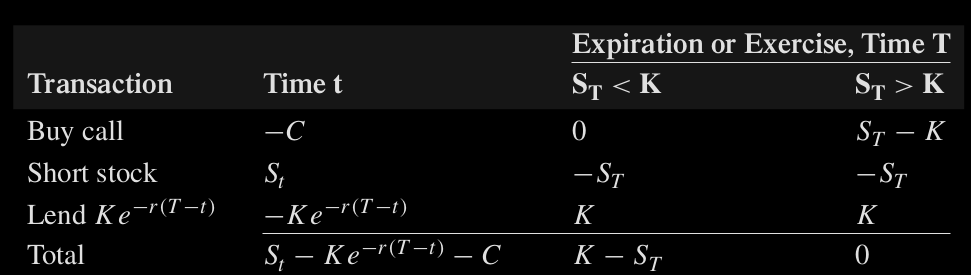
\includegraphics[scale=0.25]{figs/Table-9-4.png}

\end{center}
\end{frame}
%-------------- end slide -------------------------------%}}}
%-------------- start slide -------------------------------%{{{ 1
\begin{frame}[fragile,t]
	\frametitle{Early exercise for American options}
	\begin{center}
		Calls on stock \textcolor{cyan}{with dividends}
		\vfill

		\renewcommand{\arraystretch}{1.2}
		\begin{tabular}{|c|c|}
			\hline
			Interest beats dividends?                            & Early exercise? \\
			$K-\text{PV}_{t,T}(K) > \text{PV}_{t,T}(\text{Div})$ &                 \\ \hline
			\cmark                                               & \xmark          \\
			\xmark                                               & possibly        \\ \hline
		\end{tabular}

		\vfill

		When dividends do make early exercise rational, one should exercise \\
		at the last moment before the ex-dividend date.

	\end{center}
\end{frame}
%-------------- end slide -------------------------------%}}}
%-------------- start slide -------------------------------%{{{ 1
\begin{frame}[fragile,t]
	\begin{center}
		Early exercise for puts\\
		(no dividend case)
		\bigskip

		In order to receive interest, one may exercise early \\
		(think about the case when $S_T=0$)

		\bigskip

		\renewcommand{\arraystretch}{1.2}
		\begin{tabular}{cc}
			No early exercise & Early exercise \\ \hline
			$PV_{t,T}(K)$     & $K$            \\
		\end{tabular}

	\end{center}
\end{frame}
%-------------- end slide -------------------------------%}}}
%-------------- start slide -------------------------------%{{{ 1
\begin{frame}[fragile,t]
	\begin{center}
		Early exercise for puts\\
		(no dividend case)
		\bigskip


		No-exercise condition:
		\bigskip

		\begin{gather*}
			\textcolor{magenta}{P\left(S_t,K,T-t\right) > K -S_t} \\[1em]
			\Updownarrow                                          \\[1em]
			\textcolor{cyan}{C\left(S_t,K,T-t\right) > K - \text{PV}_{t,T}(K)}
		\end{gather*}

		\bigskip
		\mySeparateLine
		\bigskip

		\begin{equation*}
			P(S_t,K,T-t) = C(S_t,K,T-t) - S_t + \text{PV}_{t,T}(K)
		\end{equation*}
	\end{center}
\end{frame}
%-------------- end slide -------------------------------%}}}
%-------------- start slide -------------------------------%{{{ 1
\begin{frame}[fragile]
	\begin{center}
\renewcommand{\arraystretch}{1.2}
		\begin{tabular}{|c|cc|}
			\hline
                                    & calls                                     & puts                                  \\ \hline
			Receive                       & stock                                     & cash                                  \\
			Motivation for early exercise & \textcolor{magenta}{sufficient dividends} & \textcolor{cyan}{sufficient interest} \\ \hline
		\end{tabular}
		\bigskip
		\bigskip

		One can view interest as the dividend on cash. \\

		\bigskip
		Dividends are the sole reason to early-exercise an option.
	\end{center}
\end{frame}
%-------------- end slide -------------------------------%}}}
%-------------- start slide -------------------------------%{{{ 1
\begin{frame}[fragile]
	\frametitle{Time to expiration \\  -- the $K$ fixed}
	\begin{center}
		The longer the \textcolor{magenta}{more expensive}
		\bigskip

		\pause
		\begin{minipage}{0.7\textwidth}
			\begin{itemize}
				\item American call/put options
				\item European call option on stock with no dividend
					\begin{equation*}
						C_{Eur} = C_{Ame}
					\end{equation*}
			\end{itemize}
		\end{minipage}
	\end{center}

	\pause
	\mySeparateLine
	\bigskip
	\begin{center}
		The longer, might be \textcolor{cyan}{cheaper}
		\bigskip

		\pause
		\begin{minipage}{0.7\textwidth}
			\begin{itemize}
				\item European call option on stock with dividend
				\item European put option
			\end{itemize}
		\end{minipage}
	\end{center}
\end{frame}
%-------------- end slide -------------------------------%}}}
%-------------- start slide -------------------------------%{{{ 1
\begin{frame}[fragile]
	\frametitle{Time to expiration \\  -- $K_t=k e^{rt}$}

	\begin{mythm}
		When $K_t=e^{rt} K$, i.e., the strike grows at the interest rate, the premiums on European calls
		and puts on a non-dividend-paying stock increases with time to maturity.
	\end{mythm}
	\bigskip
	\pause
	\begin{myproof} We only prove the case for puts and leave the calls as exercise. \\
		Let $T>t$. In order to show that
	  \begin{align*}
		 	 P_{\text{Euro}}(S_T, K_T, T) > P_{\text{Euro}}(S_t, K_t, t),
		\end{align*}
		it suffices to find an arbitrage when
	  \begin{align*}
		 	 P_{\text{Euro}}(S_T, K_T, T) \le P_{\text{Euro}}(S_t, K_t, t).
		\end{align*}
	\end{myproof}
\end{frame}
%-------------- end slide -------------------------------%}}}
%-------------- start slide -------------------------------%{{{ 1
\begin{frame}[fragile,t]
	\begin{myproof}[ (continued)] \\
		\begin{center}
			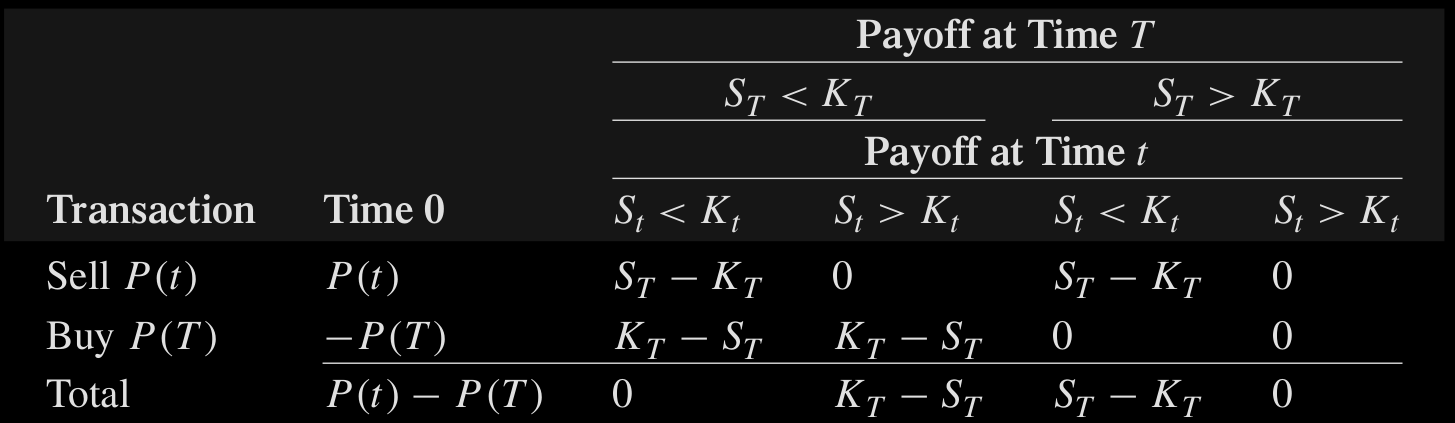
\includegraphics[scale=0.2]{figs/Table-9-5.png}
		\end{center}
		\bigskip

		For example, at time $t$, if $S_t<K_t$, one has to buy the stock. The payoff at time $t$ is
		\begin{equation*}
			S_t - K_t = S_t - K e^{rt}
		\end{equation*}
		One keeps this stock to time $T$, the stock price becomes  $S_T$, and the future value of
		$Ke^{rt}$ that one spent at time $t$ becomes  $Ke^{rt + r(T-t)}=Ke^{rT}$. Hence, the payoff of
		this strategy at time $T$ is
		\begin{equation*}
			S_T - Ke^{rT} = S_T - K_T.
		\end{equation*}
		\myEnd
	\end{myproof}
\end{frame}
%-------------- end slide -------------------------------%}}}
%-------------- start slide -------------------------------%{{{ 1
\begin{frame}[fragile,t]
	\frametitle{Different strike prices}
	\begin{center}
		$ K_1\le K_2 \le K_3$\\
		\bigskip

		\renewcommand{\arraystretch}{2.5}
		\begin{tabular}{|c|c|}
			\hline
			Relation                                                                         & Ideas in proof, arbitrage in          \\ \hline
			$C(K_1) \ge C(K_2)$                                                              & a call \textcolor{green}{bull} spread \\
			$P(K_1) \le P(K_2)$                                                              & a put \textcolor{red}{bear} spread    \\ \hline
			$C(K_1)-C(K_2) \le K_2-K_1$                                                      & a call \textcolor{red}{bear} spread   \\
			$P(K_2)-P(K_1) \le K_2-K_1$                                                      & a put \textcolor{green}{bull} spread  \\ \hline
			$ \displaystyle \frac{C(K_1)-C(K_2)}{K_2-K_1} \ge \frac{C(K_2)-C(K_3)}{K_3-K_2}$ & an asymmetric butterfly spread        \\
			$ \displaystyle \frac{P(K_2)-P(K_1)}{K_2-K_1} \le \frac{P(K_3)-P(K_2)}{K_3-K_2}$ & an asymmetric butterfly spread        \\ \hline
		\end{tabular}
	\end{center}
\end{frame}
%-------------- end slide -------------------------------%}}}
%-------------- start slide -------------------------------%{{{ 1
\begin{frame}[fragile,t]
\begin{center}
	Convexity revisited

	\begin{gather*}
		\frac{C(K_1)-C(K_2)}{K_2-K_1} \ge \frac{C(K_2)-C(K_3)}{K_3-K_2} \\[1em] \Updownarrow \\[1em]
		 C(K_2) \ge \lambda C(K_1) + (1-\lambda) C(K_3).
	\end{gather*}
	with
	\begin{align*}
		\lambda = \frac{K_3-K_2}{K_3-K_1}
	\end{align*}
\end{center}
\end{frame}
%-------------- end slide -------------------------------%}}}
%-------------- start slide -------------------------------%{{{ 1
\begin{frame}[fragile,t]
\begin{myexample}
	Suppose that
	\begin{center}
		\renewcommand{\arraystretch}{1.2}
		\begin{tabular}{ccc}
			Strike       & 50 & 55 \\
			Call Premium & 18 & 12 \\
		\end{tabular}
		\begin{enumerate}
			\item What no-arbitrage property is violated?
			\item What spread position would you use to effect arbitrage?
			\item Demonstrate that the spread position is an arbitrage.
		\end{enumerate}
	\end{center}
\end{myexample}
\pause
\bigskip
\begin{mysol}
	\textcolor{gray}{Check Example 9.4 on p. 283.} \myEnd
\end{mysol}
\end{frame}
%-------------- end slide -------------------------------%}}}
%-------------- start slide -------------------------------%{{{ 1
\begin{frame}[fragile,t]
\begin{myexample}
	Suppose that
	\begin{center}
		\renewcommand{\arraystretch}{1.2}
		\begin{tabular}{cccc}
			Strike       & 50 & 59  & 65 \\
			Call premium & 14 & 8.9 & 5  \\
		\end{tabular}
		\begin{enumerate}
			\item What no-arbitrage property is violated?
			\item What spread position would you use to effect arbitrage?
			\item Demonstrate that the spread position is an arbitrage.
		\end{enumerate}
	\end{center}
\end{myexample}
\pause
\bigskip
\begin{mysol}
	\textcolor{gray}{Check Example 9.5 on p. 284.} \myEnd
\end{mysol}
\end{frame}
%-------------- end slide -------------------------------%}}}
%-------------- start slide -------------------------------%{{{ 1
\begin{frame}[fragile,t]
\begin{myexample}
	Suppose that
	\begin{center}
		\renewcommand{\arraystretch}{1.2}
		\begin{tabular}{cccc}
			Strike      & 50 & 55 & 70 \\
			Put premium & 4  & 8  & 16 \\
		\end{tabular}
		\begin{enumerate}
			\item What no-arbitrage property is violated?
			\item What spread position would you use to effect arbitrage?
			\item Demonstrate that the spread position is an arbitrage.
		\end{enumerate}
	\end{center}
\end{myexample}
\pause
\bigskip
\begin{mysol}
	\textcolor{gray}{Check Example 9.6 on p. 284.} \myEnd
\end{mysol}
\end{frame}
%-------------- end slide -------------------------------%}}}


\def\mySecNum{9.4}
\mySection{\mySecNum~Problems}
%-------------- start slide -------------------------------%{{{ 1
\begin{frame}[fragile,t]
	Problems:
	9.1,
	9.2,
	9.3,
	9.4,
	9.8,
	9.9,
	9.10,
	9.11,
	9.15.
	% 5.11,
	% 5.12,
	% 5.16,
	% 5.20.
	\\
	\bigskip

	Due Date: TBA
\end{frame}
%-------------- end slide -------------------------------%}}}

\end{document}
